% Versión para diapositiva (plantilla Semana ICG 2026): tamaño real 1:1, texto de 24 pt.
% Proceso 2 (proceso2mosaico.ipynb). Insertar en PowerPoint al 100 %.
\documentclass[border=2pt]{standalone}
\usepackage{iftex}
\ifPDFTeX
  \usepackage[utf8]{inputenc}
  \usepackage[T1]{fontenc}
  \usepackage[sfdefault]{carlito}
\else
  \usepackage{fontspec}
  \setmainfont{Carlito}[Extension=.ttf, UprightFont=*-Regular, BoldFont=*-Bold,
    ItalicFont=*-Italic, BoldItalicFont=*-BoldItalic]
\fi
\usepackage{tikz}
\usetikzlibrary{arrows.meta, positioning, fit, backgrounds}

\definecolor{tinta}{HTML}{1B2A3A}
\definecolor{azul}{HTML}{1D5F83}
\definecolor{azulosc}{HTML}{164A66}
\definecolor{verde}{HTML}{5E8C45}

\begin{document}
\fontsize{24}{29}\selectfont
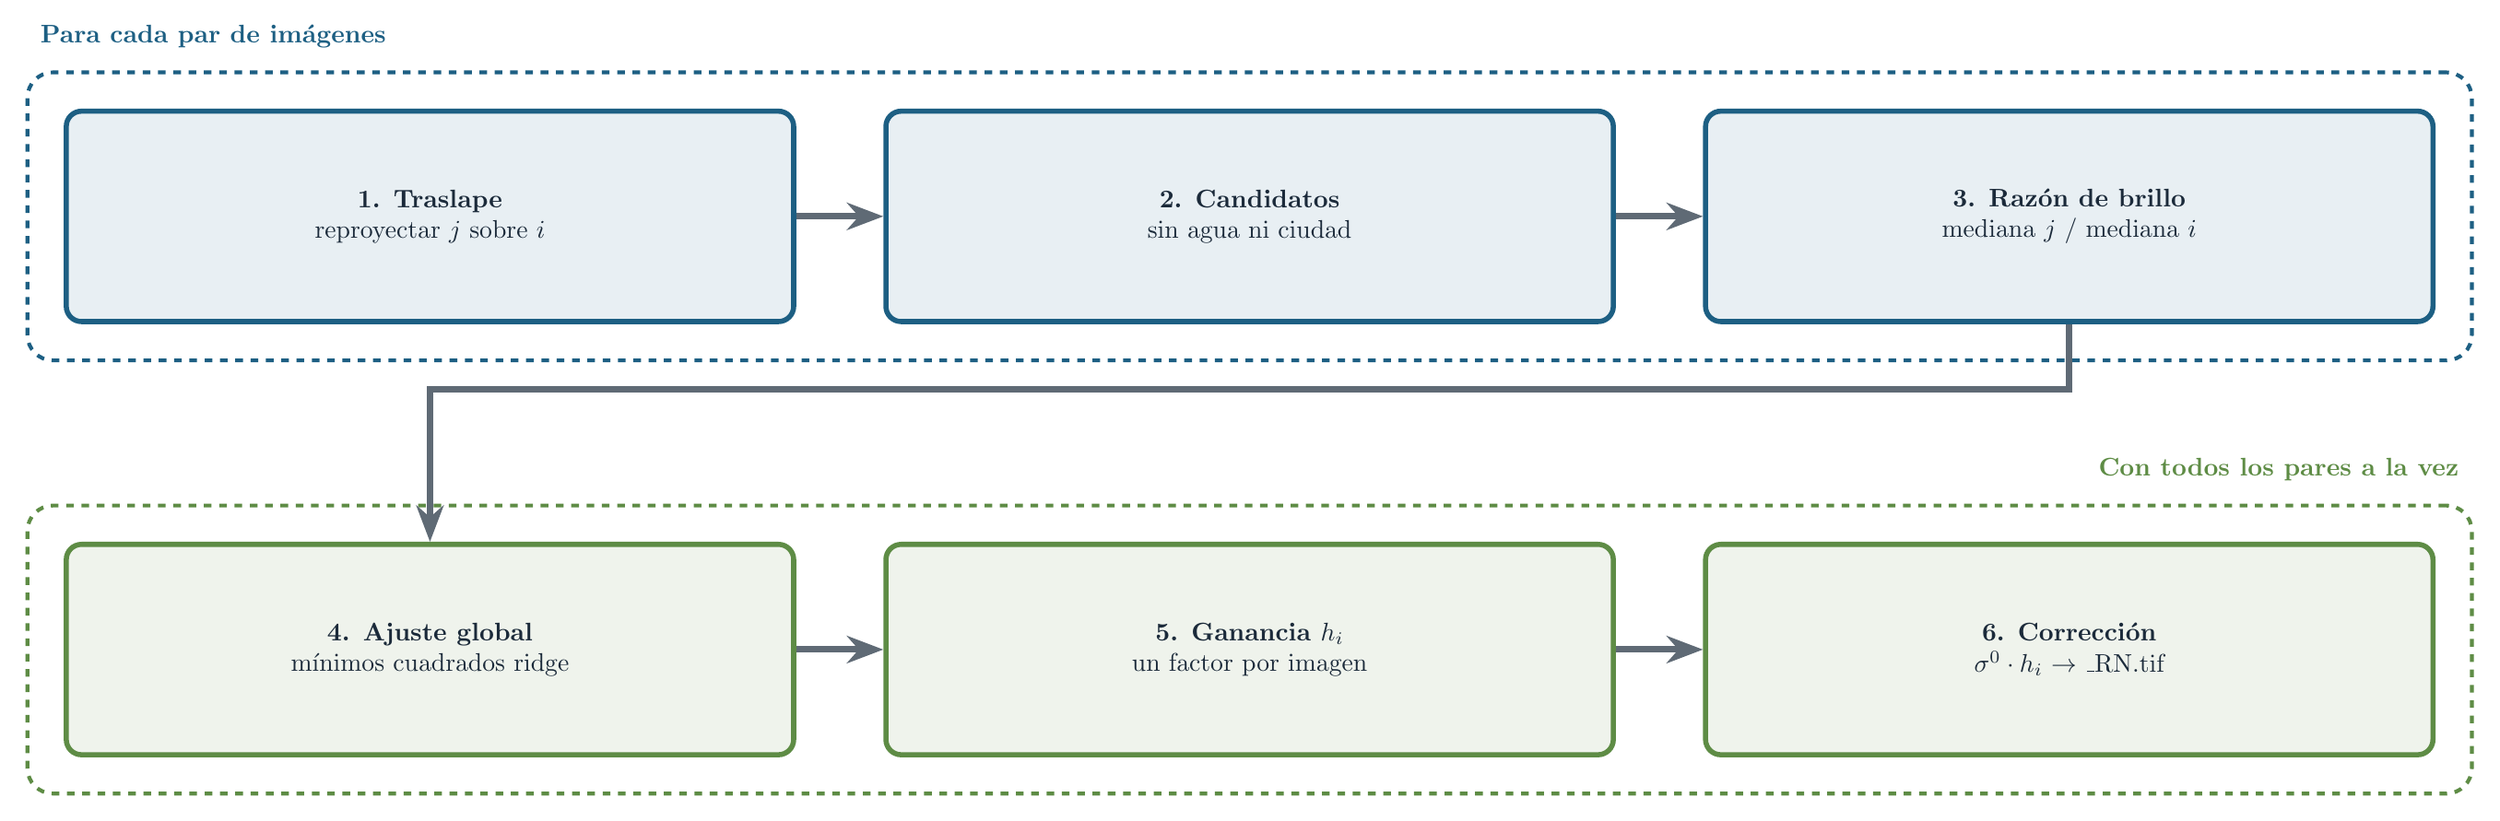
\begin{tikzpicture}[
  >=Stealth,
  paso/.style={rectangle, rounded corners=6pt, draw=#1, line width=2pt,
               fill=#1!10, text width=9.6cm, minimum height=2.9cm,
               align=flush center, text=tinta, inner sep=6pt},
  grupo/.style={draw=#1, dashed, line width=1.5pt, rounded corners=10pt,
                inner xsep=5mm, inner ysep=5mm},
  etq/.style={anchor=south west, font=\bfseries, text=#1, inner sep=0pt},
  flecha/.style={->, line width=2.5pt, draw=tinta!70}
]
% fila 1: por pares
\node[paso=azul] (p1) {\textbf{1. Traslape}\\ reproyectar $j$ sobre $i$};
\node[paso=azul, right=12mm of p1] (p2) {\textbf{2. Candidatos}\\ sin agua ni ciudad};
\node[paso=azul, right=12mm of p2] (p3) {\textbf{3. Razón de brillo}\\ mediana $j$ / mediana $i$};
% fila 2: global
\node[paso=verde, below=30mm of p1] (p4) {\textbf{4. Ajuste global}\\ mínimos cuadrados ridge};
\node[paso=verde, right=12mm of p4] (p5) {\textbf{5. Ganancia $h_i$}\\ un factor por imagen};
\node[paso=verde, right=12mm of p5] (p6) {\textbf{6. Corrección}\\ $\sigma^0 \cdot h_i$ $\rightarrow$ \_RN.tif};

\begin{scope}[on background layer]
  \node[grupo=azul,  fit=(p1)(p3)] (g1) {};
  \node[grupo=verde, fit=(p4)(p6)] (g2) {};
\end{scope}
\node[etq=azul]  at ([xshift=2mm, yshift=3mm]g1.north west) {Para cada par de imágenes};
\node[etq=verde, anchor=south east] at ([xshift=-2mm, yshift=3mm]g2.north east) {Con todos los pares a la vez};

\foreach \a/\b in {p1/p2, p2/p3, p4/p5, p5/p6}
  \draw[flecha] (\a.east) -- (\b.west);
\draw[flecha] (p3.south) -- ++(0,-9mm) -| (p4.north);
\end{tikzpicture}
\end{document}
